In order to achieve better performance than the algorithms described in subsection 3.3, we decided to proceed with changing both the classification algorithm and the vectorizer used both for experimentation and performance optimization.

\subsubsection{Vectorizer}
For this architecture we used Python's scikit-learn HashingVectorizer. HashingVectorizer applies a hashing function to term frequency counts in each document making it an efficient way of mapping terms to features. Even though using a hash function can lead to collisions (e.g. distinct tokens mapped to the same feature index), with HashingVectorizer this is rarely an issue as there is a parameter, \textit{n\_features}, that can be tweaked to avoid collisions. The parameter \textit{n\_features} refers to the number of features (columns) in the output matrices. In our tests we tried different values for \textit{n\_features} and after many tests we decided that with the given dataset, the most performing value was \textit{n\_features}=$2^{18}$ which is the recommended one for text classification problems.

\subsubsection{Classification Algorithm}
In the shake of experimentation we decided to implement a neural network for this task. The neural network used, is a Multi-layer Perceptron classifier. A multilayer perceptron (MLP)\cite{MLP}is a class of feedforward artificial neural network. A MLP consists of, at least, three layers of nodes: an input layer, a hidden layer and an output layer. Except for the input nodes, each node is a neuron that uses a nonlinear activation function. MLP utilizes a supervised learning technique called backpropagation for training. Multilayer perceptrons are sometimes colloquially referred to as "vanilla" neural networks, especially when they have a single hidden layer. A hypothetical example of a Multilayer Perceptron Network is shown in Figure 1. 

\begin{figure}[h]
\centering
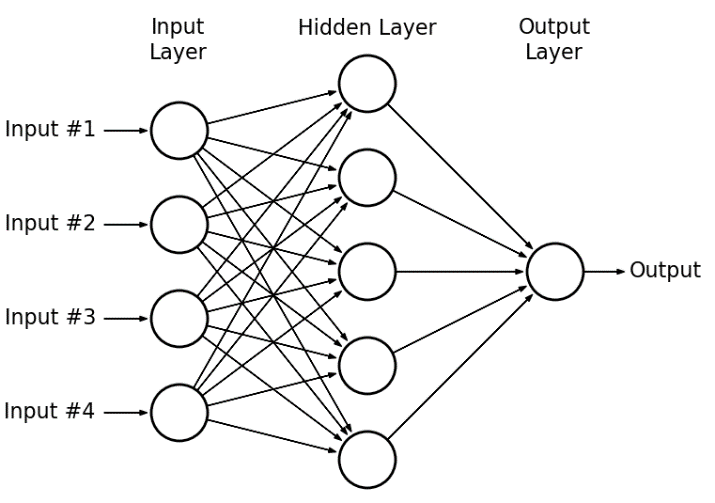
\includegraphics[scale=0.35]{images/MLP.png}
\caption{A hypothetical example of a MLP Network}
\end{figure}

\subsubsection{Performance}
In our architecture, the MLP consist of an Input Layer, a single Hidden Layer with 100 of neurons and an Output Layer. Testing the performance of the MLP, using the token vectors from \textit{HashingVectorizer} we managed to achieve a performance increase over the methods used in subsection 3.3 as shown in the total performance report file (EvaluationMetric\_10fold.csv). The performance of this architecture was consistently better as there were multiple experiments with different seeds and inputs.